\documentclass[12pt,a4paper,onecolumn]{article}
\usepackage[utf8]{inputenc}
\usepackage[T1]{fontenc}
\usepackage[french]{babel}
\usepackage{amsmath}
\usepackage{amsfonts}
\usepackage{amssymb}
\usepackage{amscd}
\usepackage{amsthm}
\usepackage{physics}
\usepackage[left=2.2cm,right=2.2cm,top=2cm,bottom=2cm]{geometry}
\usepackage{textcomp,gensymb} %pour le °C, et textcomp pour éviter les warning
\usepackage{graphicx} %pour les images
\usepackage{caption}
\usepackage{subcaption}
\usepackage[colorlinks=true,
	breaklinks=true,
	citecolor=blue,
	linkcolor=blue,
	urlcolor=blue]{hyperref} % pour insérer des liens
\usepackage{epstopdf} %converting to PDF
\usepackage[export]{adjustbox} %for large figures

\usepackage{array}
\usepackage{dsfont}% indicatrice : \mathds{1}
%\usepackage[dvipsnames]{xcolor}

% ------------------------- Blbiographie --------------------------------------
% \usepackage[backend=biber, style=science]{biblatex}
% \addbibresource{biblio.bib}
% ------------------------------------------------------------------------------

% ------------------------- Color table ----------------------------------------
\usepackage{multirow}
\usepackage[table]{xcolor}
\definecolor{maroon}{cmyk}{0,0.87,0.68,0.32}
% ------------------------------------------------------------------------------

\setcounter{tocdepth}{4} %Count paragraph
\setcounter{secnumdepth}{4} %Count paragraph
\usepackage{float}

\usepackage{graphicx} % for graphicspath
% \graphicspath{{../images/}}

\usepackage{array,tabularx}
\newcolumntype{L}[1]{>{\raggedright\let\newline\\\arraybackslash\hspace{0pt}}m{#1}}
\newcolumntype{C}[1]{>{\centering\let\newline\\\arraybackslash\hspace{0pt}}m{#1}}
\newcolumntype{R}[1]{>{\raggedleft\let\newline\\\arraybackslash\hspace{0pt}}m{#1}}

\title{Panorama construction}
\author{Vincent Matthys Maureen Muscat Mariène Wan}


\renewcommand{\thesubsection}{\alph{subsection}}


\begin{document}
%\maketitle
\begin{tabularx}{\textwidth}{@{} l X r @{} }
{\textsc{Master MVA}} & & \textsc{use scenario}\\
\textsc{UE 3D COMPUTER VISION} & &{ENS Paris Saclay}\\
%& %M1 Informatique
\end{tabularx}
\vspace{1.5cm}
\begin{center}

\rule[11pt]{5cm}{0.5pt}

\textbf{\LARGE \textsc{Panorama construction}}
\vspace{0.5cm}

Vincent Matthys


\rule{5cm}{0.5pt}

\vspace{1.5cm}
\end{center}

\section{Objective}
This program allows the user to reconstruct a scene from two images, when the two images comes from a static scene with 2 different views, which are overlapping over a certain area, in the following particular conditions :
\begin{itemize}
\item the observed scene is flat
\item the observed scene is not flat, but the two views differs only from a rotation around the optical center and change of internal parameters of camera.
\end{itemize}
The user is asked to select sequentially matching points of both images. Then the program builds the panorama, and saves it in the folder of current program execution. The program ends with any user click after the construction of the panorama.

\section{Material \& Method}
A single C++ file, named \textit{Panorama.cpp} loads and displays two images, which can be passed in arguments to the program named \textit{Panorama}. The coordinates of matching points ($(x_i, y_i)$ matching for $(x_i^{\prime}, y_i^{\prime})$) are used to reconstruct the homography between the two images, solving the following linear system :
$$
\begin{bmatrix}
\vdots & \vdots & \vdots & \vdots & \vdots & \vdots & \vdots & \vdots\\
x_i & y_i & 1 & 0 & 0 & 0 & -x_i^{\prime}x_i & -x_i^{\prime}y_i\\
0 & 0 & 0 & x_i & y_i & 1 & -y_i^{\prime}x_i & -y_i^{\prime}y_i\\
\vdots & \vdots & \vdots & \vdots & \vdots & \vdots & \vdots & \vdots
\end{bmatrix}
\dotproduct
\begin{bmatrix}
h_{11}\\
h_{12}\\
h_{13}\\
h_{21}\\
h_{22}\\
h_{23}\\
h_{31}\\
h_{32}\\
\end{bmatrix}
=
\begin{bmatrix}
\vdots \\
x_i^{\prime}\\
y_i^{\prime}\\
\vdots
\end{bmatrix}
$$
where the $h_{ij}$ are the homography values, for $h_{33}$ arbitrary set to 1, without loss of generality.

$$ H =
\begin{bmatrix}
h_{11} & h_{12} & h_{13}\\
h_{21} & h_{22} & h_{23}\\
h_{31} & h_{32} & 1
\end{bmatrix}
$$

To successfully finds H, the system requires at least 4 correspondences, each one giving two equations. If there is more than 4 correspondences, the program solves the system using least squares programming.
A sanity check is introduced and allows user the homography found. Every line should be $(0, 0, 0)$ vector. In reality, it is only close to the null vector, because, in particular, of errors during selection of points and the intrinsic noise of the camera.

To build the panorama, the program uses the pull method, which requires to inverse the homography, and queries the preimage by H, which is the image by H, of each pixel in the final image. If it lies in the first image, then the pixel is pulled in the final image. In the overlapping area, the program simply averages the value of the two images.

\section{Results}
We present here 3 use cases obtained with the default images :
\begin{enumerate}
\item first view, left of the scene. Size : 755 x 499
\item second view, right of the scene. Size : 755 x 499
\end{enumerate}

\subsection{Wrong use case}

\subsubsection{Not enough correspondences}

When the user doesn't give enough correspondences, the sanity check doesn't display, since the linear system can't be solved. Moreover, the homography is given, by default, as the identity matrix. Hence the panorama constructed in figure \ref{not_enough} is only the average of both image, as if they were taken with the same view.
\begin{figure}[H]
\begin{center}
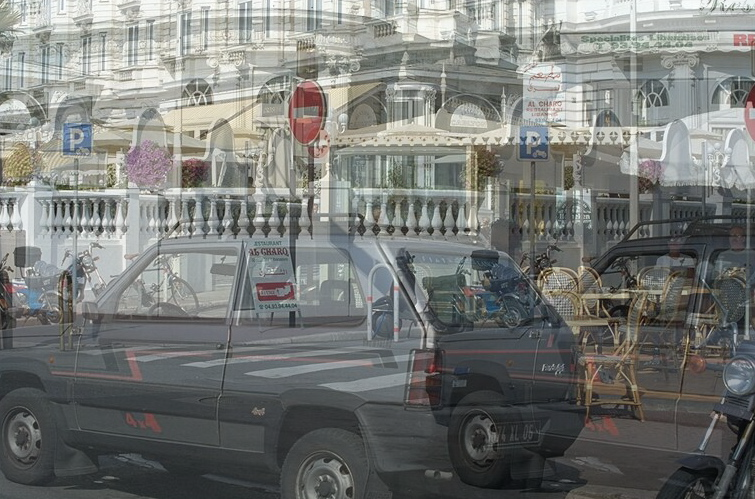
\includegraphics[width = \textwidth]{panorama_not_enough.png}
\end{center}
\caption{Panorama construction with not enough correspondences. Size : 755 x 499}
\label{not_enough}
\end{figure}

\subsubsection{Wrong correspondences}

When the user doesn't take proper correspondances, the homography found relies on wrong correspondances, hence a obvious wrong panorama construction, with geometric deformations.
In the case presented in figure \ref{wrong_corr}, we can see those deformations and the homography found is the following :

$$ H =
\begin{bmatrix}
0.792 & -0.281 & -279\\
-0.040 & 0.250 & 100\\
0.00 & 0.00 & 1
\end{bmatrix}
$$

\begin{figure}[H]
\begin{center}
\frame{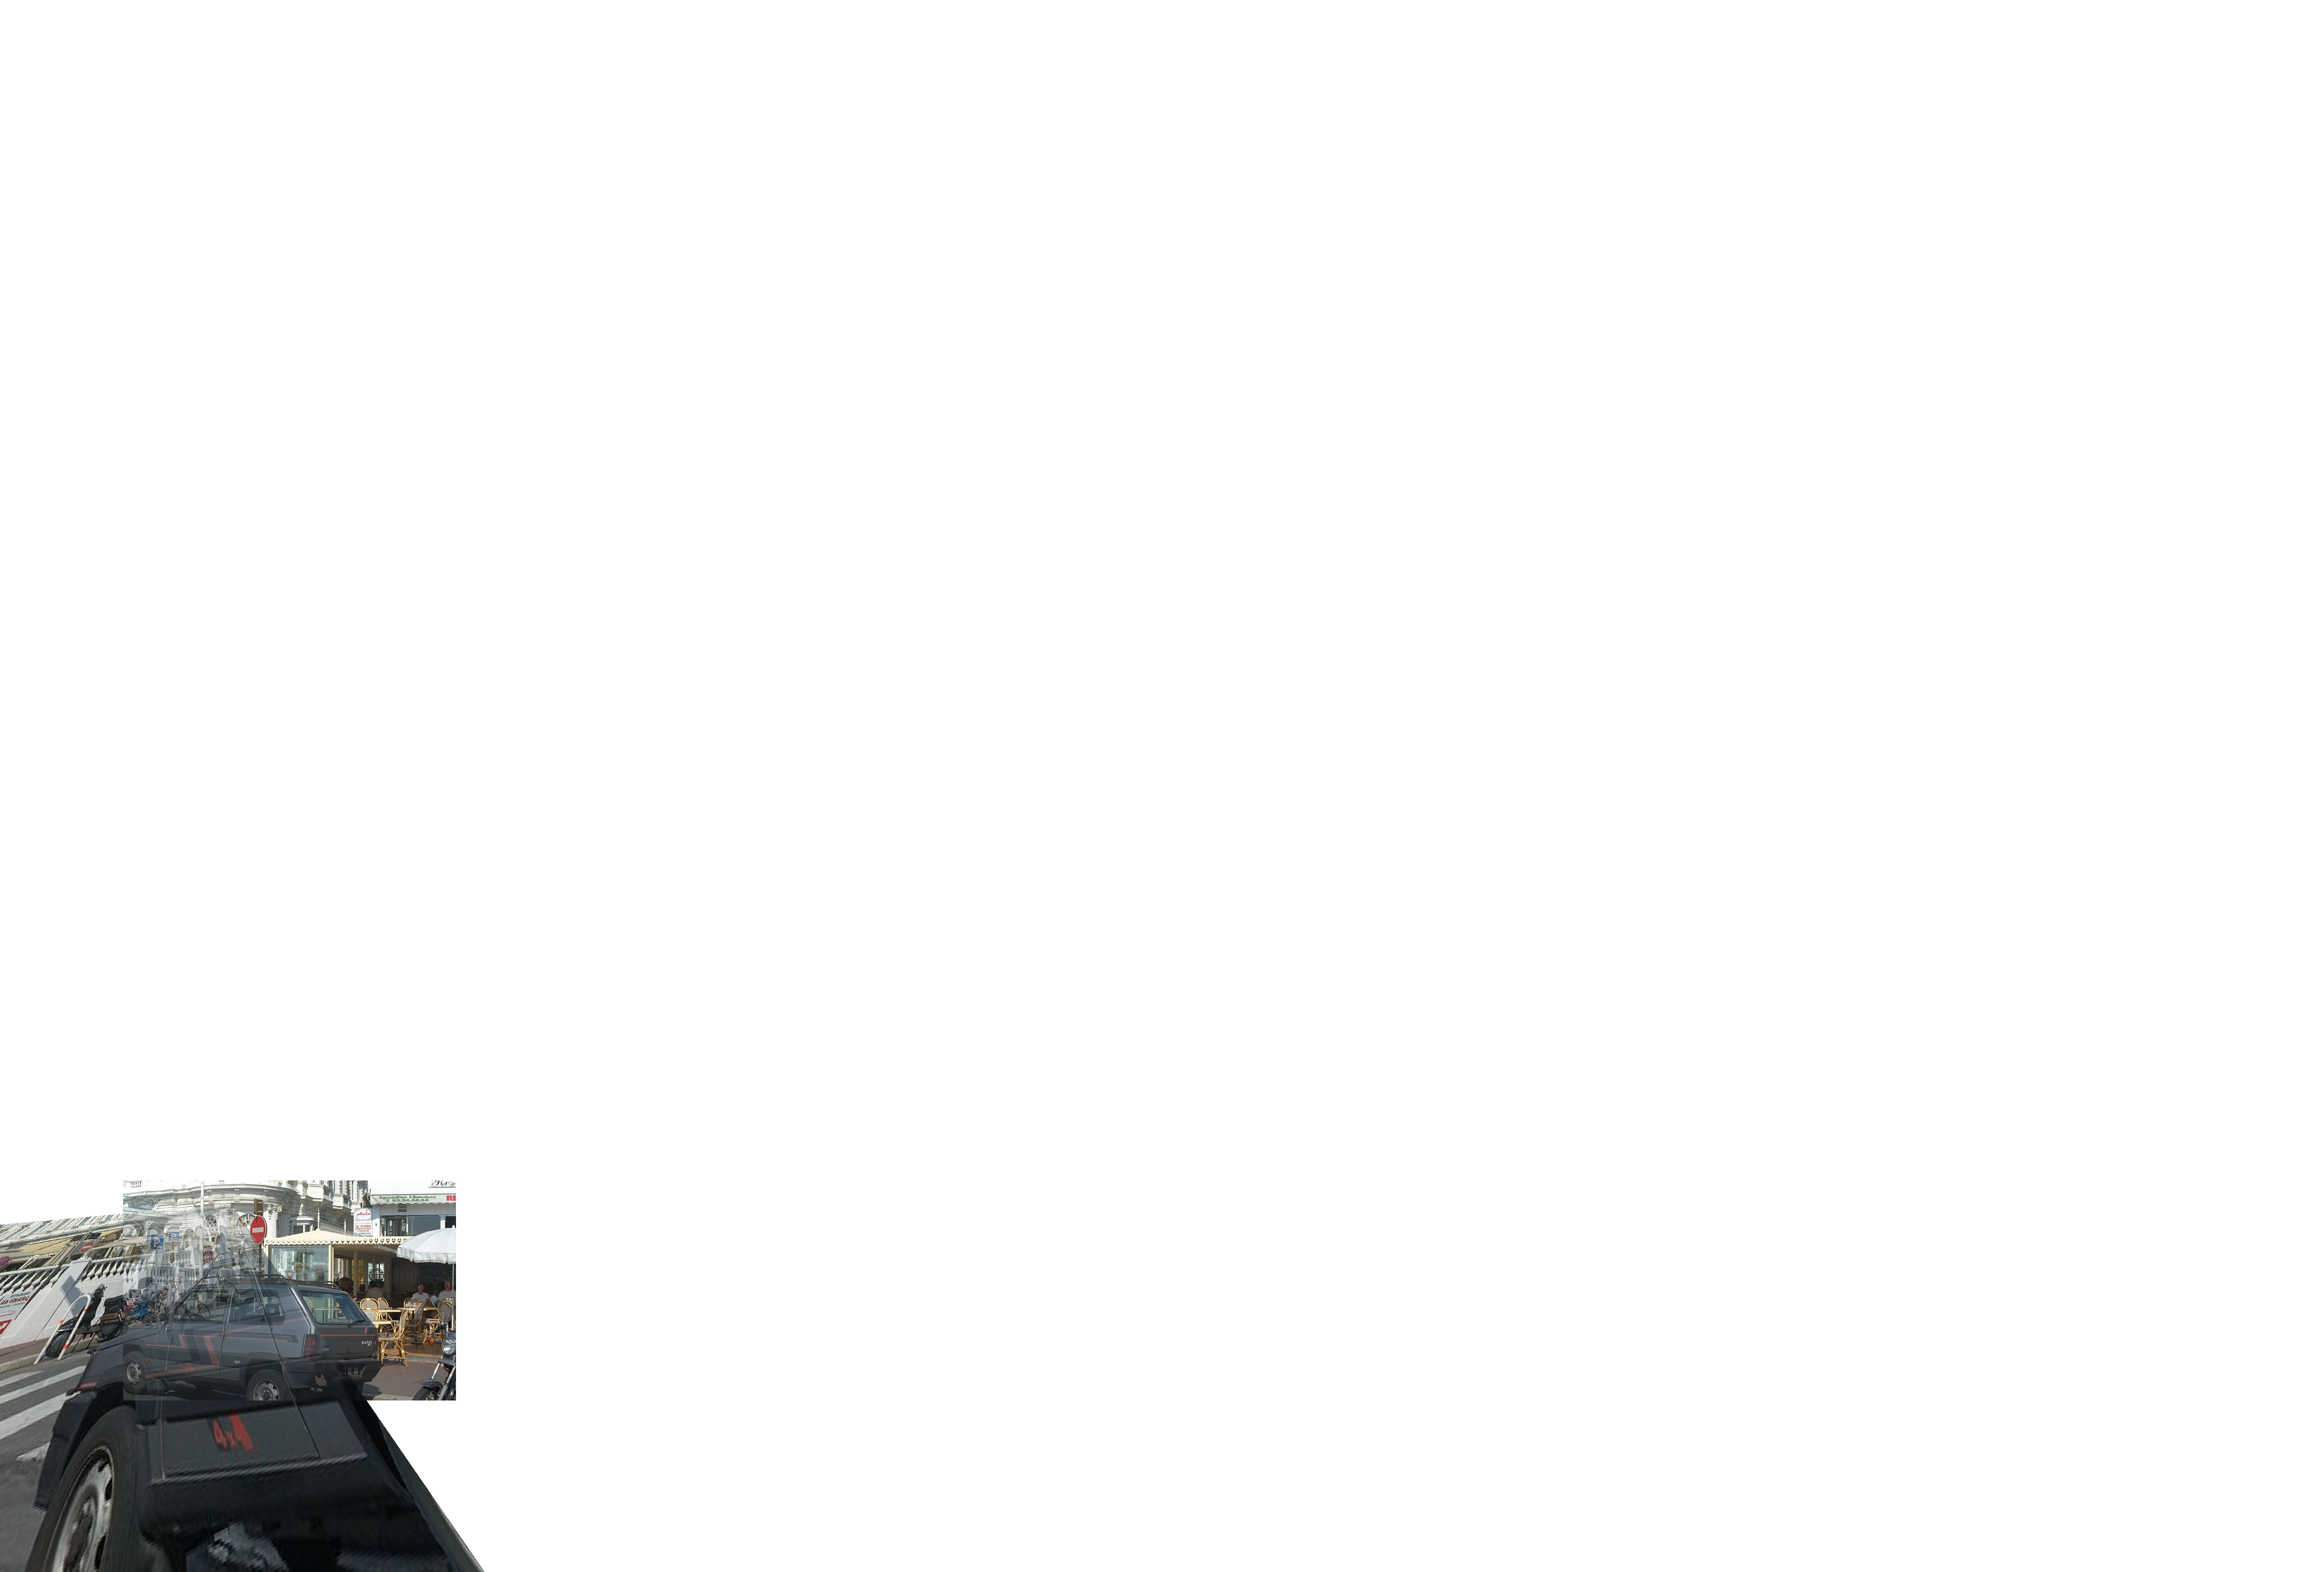
\includegraphics[width = \textwidth]{panorama_wrong_corr.png}}
\end{center}
\caption{Panorama construction with obvious wrong correspondences. A frame has been added to see the image size of the panorama : 5270 x 3565}
\label{wrong_corr}
\end{figure}

\subsection{With 4 correspondences}

In figure \ref{mini_corr}, a minimum number of 4 correspondences allows to find a proper homography between the two views. The overlapping area still remains a little blurred, and the panorama construction highlights is not rectangular, which shows that the homography found, given below is not perfect. Moreover, we can notice some aliasing on vertical lines on the pulled image.

$$ H =
\begin{bmatrix}
1.02 & 7.36e-5 & -468\\
0.0120 & 1.02 & -8\\
0.00 & 0.00 & 1
\end{bmatrix}
$$

\begin{figure}[H]
\begin{center}
\begin{tabular}{p{0.5\textwidth}  p{0.5\textwidth}}
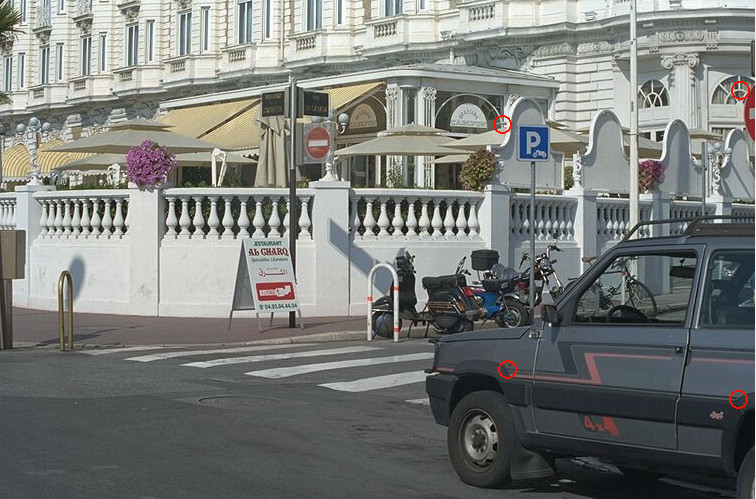
\includegraphics[width = 0.5\textwidth]{I1_2.png} &
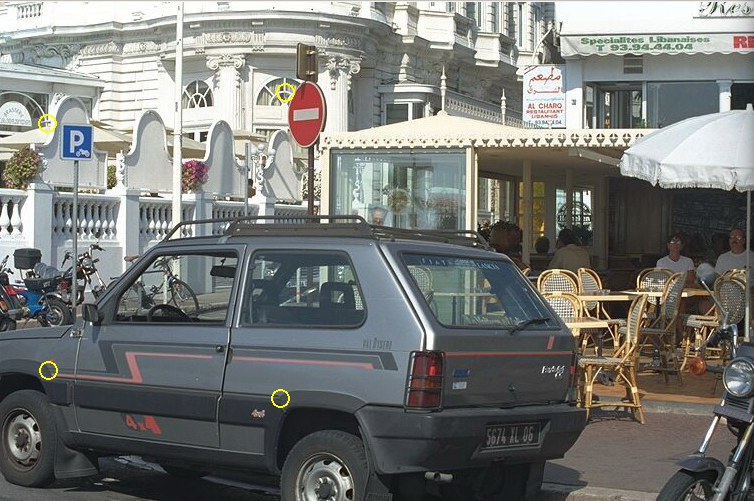
\includegraphics[width = 0.5\textwidth]{I2_2.png} \\
\multicolumn{2}{c}{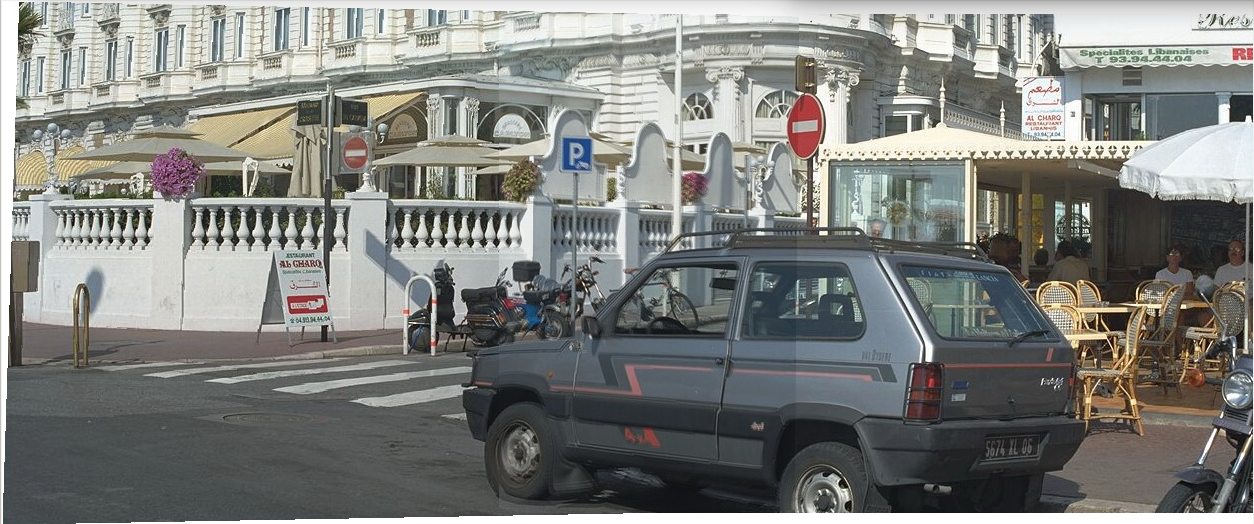
\includegraphics[width = 1.0\textwidth]{Panorama_2.png}}
\end{tabular}
\end{center}
\caption{Top left : first view of the scene. Top right : second view of the scene. Top : circles highlight the correspondances. Bottom : panorama construction with the given correspondances. Size : 1254 x 524}
\label{mini_corr}
\end{figure}

\subsection{With more than 4 correspondanecs}

In figure \ref{many_corr}, 10 correspondences allow to find an almost perfect homography between the two views. The overlapping area is nearly not blurred, and the panorama format is almost rectangular, which corresponds to a rotation of the view between the optical center.

\subsection{With 4 correspondances}
\begin{figure}[H]
\begin{center}
\begin{tabular}{p{0.5\textwidth}  p{0.5\textwidth}}
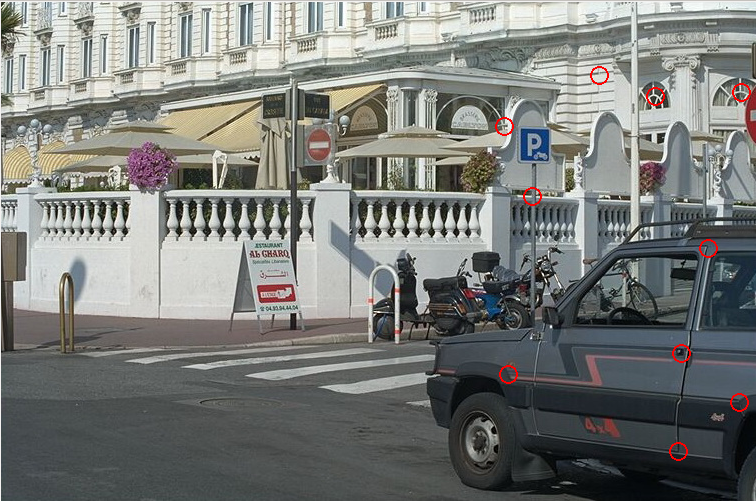
\includegraphics[width = 0.5\textwidth]{I1_3.png} &
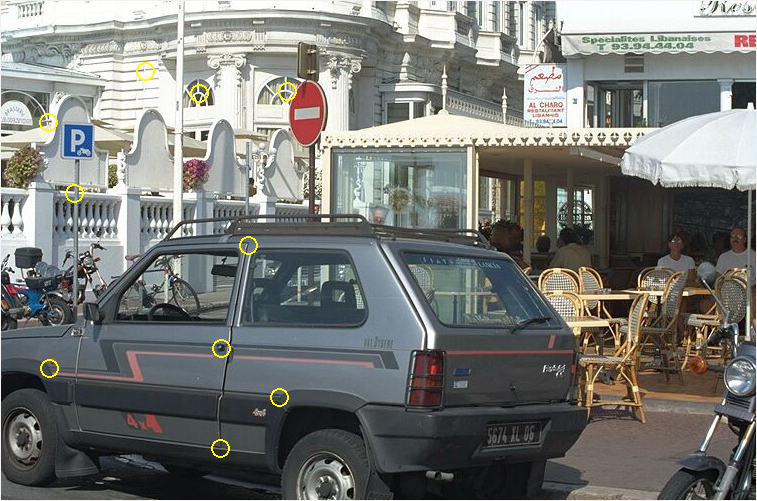
\includegraphics[width = 0.5\textwidth]{I2_3.png} \\
\multicolumn{2}{c}{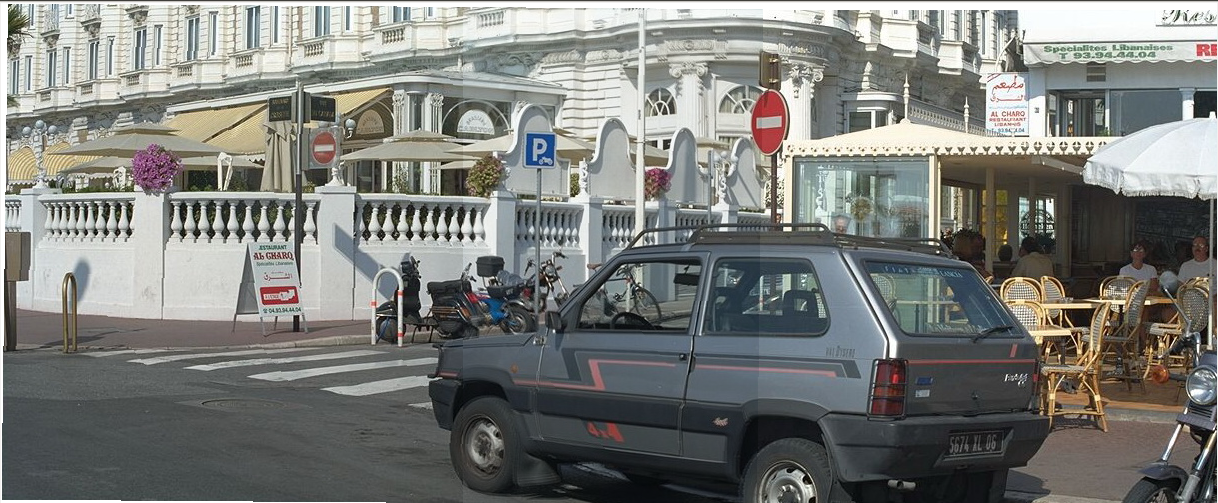
\includegraphics[width = 1.0\textwidth]{Panorama_3.png}}
\end{tabular}
\end{center}
\caption{Top left : first view of the scene. Top right : second view of the scene. Top : circles highlight the correspondances. Bottom : panorama construction with the given correspondances. Size : 1218 x 503}
\label{many_corr}
\end{figure}

\end{document}
